\documentclass[conference]{IEEEtran}
\IEEEoverridecommandlockouts
\usepackage[utf8]{inputenc}
\usepackage[spanish,es-nodecimaldot]{babel}
\usepackage{cite}
\usepackage{amsmath,amssymb,amsfonts}
\usepackage{graphicx}
\graphicspath{{./}{figures/}{report/}}
\usepackage{xcolor}
\usepackage{booktabs}
\usepackage{hyperref}
\begin{document}

\title{Reconocimiento de Comandos de Voz en Español con un Autoencoder de Reducción de Ruido (Avance)}

\author{\IEEEauthorblockN{Facundo Bautista Barbera}
\IEEEauthorblockA{\textit{Escuela de Ingeniería y Ciencias} \\
\textit{Instituto Tecnológico y de Estudios Superiores de Monterrey}\\
A01066843@tec.mx}
}

\maketitle

\begin{abstract}
Resumen pendiente.
\end{abstract}

\begin{IEEEkeywords}
reconocimiento de comandos de voz, autoencoder, aprendizaje multitarea, espectrograma log-mel, robustez al ruido
\end{IEEEkeywords}

\section{Introducción}
Reconocer palabras clave habladas es la base de las interfaces de voz: un dispositivo escucha un flujo de audio continuo y solo reacciona cuando detecta una palabra de interés. Con audio limpio el problema se resuelve bien con una red convolucional pequeña \cite{b1}, pero en la práctica el audio llega con ruido de fondo y la exactitud disminuye de forma notable cuando el ruido tiene un volumen comparable al de la voz.

Una forma de mejorar la robustez es entrenar la red para que, además de clasificar, reconstruya el espectrograma limpio a partir del ruidoso, como lo hace un autoencoder de reducción de ruido \cite{b4}. Si el codificador compartido aprende a separar la voz del ruido para poder reconstruir, esa representación también puede beneficiar al clasificador. Este enfoque corresponde al aprendizaje multitarea \cite{b6}, en el que una sola red persigue dos objetivos que comparten parte de sus parámetros.

El vocabulario está formado por los diez dígitos y diez comandos para una interfaz de voz: siguiente, anterior, música, alto, sigue, adelante, arriba, abajo, izquierda y derecha. A diferencia de conjuntos en inglés como Speech Commands \cite{b7}, no fue posible incluir ``sí'' y ``no'' porque el corpus descarta las palabras de menos de tres letras.

\section{Descripción de los datos}
\subsection{Voz: Multilingual Spoken Words Corpus}
Los clips de voz provienen de la parte en español del Multilingual Spoken Words Corpus (MSWC) \cite{b2}, construido a partir de grabaciones de Common Voice. Su tabla de clips contiene 1208209 clips de 24878 palabras distintas, dichas por 12461 hablantes, con una partición oficial de 78.2\% entrenamiento, 10.9\% desarrollo (dev) y 10.9\% prueba. El audio se distribuye en formato Opus a 48 kHz y los clips ya tienen una duración cercana a un segundo.

La distribución de clips por palabra es muy desigual, como muestra la Figura~\ref{fig:rank}: la mitad de las palabras del corpus tiene 11 clips o menos. Los dígitos cuentan con miles de clips, por ejemplo ``dos'' con 6211, mientras que los comandos menos frecuentes tienen unos cientos: ``derecha'' tiene 170 e ``izquierda'' y ``abajo'' 174 cada una.

\begin{figure}[htbp]
\centering
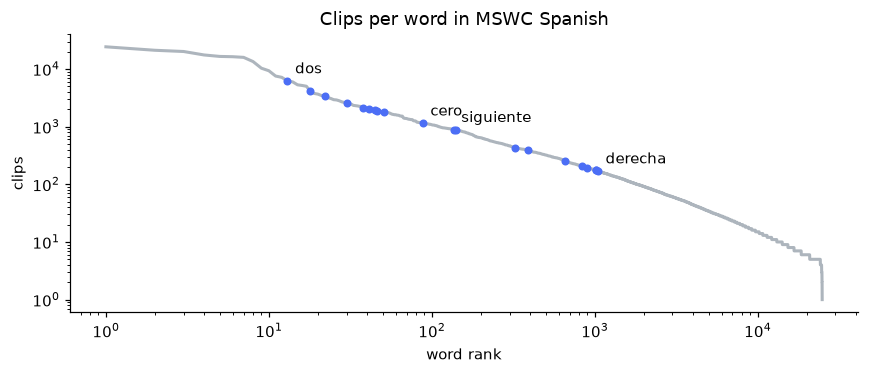
\includegraphics[width=\columnwidth]{palabras_rank.png}
\caption{Clips por palabra en MSWC en español (ejes logarítmicos), con las 20 palabras del vocabulario marcadas.}
\label{fig:rank}
\end{figure}

\subsection{Ruido: ESC-50}
El ruido de fondo proviene de ESC-50 \cite{b3}, un conjunto de 2000 grabaciones de 5 segundos de 50 categorías de sonidos ambientales, como lluvia, aviones, lavadoras o aspiradoras. El conjunto ya viene dividido en cinco folds. Los folds 1 a 3 se usan para entrenamiento, el fold 4 para validación y el fold 5 para prueba, de modo que el ruido con el que se evalúa el modelo no se observa durante el entrenamiento ni durante la selección del mejor punto de control.

\section{Preparación de los datos}
\subsection{Selección de clips y clases}
Para equilibrar las clases, cada palabra se limita a 1500 clips de entrenamiento y 200 de dev y de prueba. Se agregan dos clases adicionales para llegar a 22. La clase \textit{unknown} reúne otras palabras del corpus, con un máximo de 2 clips por palabra y 2500, 300 y 300 clips en los tres splits, para que el modelo aprenda a rechazar voz que no corresponde a un comando. La clase \textit{silence} consiste en clips sin señal, 1000, 150 y 150 por split, a los que se les agrega ruido durante el entrenamiento. Estas dos clases son necesarias porque en uso real el modelo escucha un flujo continuo en el que la mayor parte del tiempo no hay un comando. El resultado son 20875 clips de entrenamiento, 2707 de dev y 2707 de prueba (Tabla~\ref{tab:clases}).

\begin{table}[htbp]
\caption{Clips por clase y por split (entrenamiento / dev / prueba)}
\label{tab:clases}
\centering
\small
\setlength{\tabcolsep}{3pt}
\begin{tabular}{lc@{\hspace{1em}}lc}
\toprule
Clase & Clips & Clase & Clips \\
\midrule
cero & 920/115/115 & siguiente & 710/89/89 \\
uno & 1500/200/200 & anterior & 206/26/26 \\
dos & 1500/200/200 & música & 700/88/88 \\
tres & 1500/200/200 & alto & 312/39/39 \\
cuatro & 1500/200/200 & sigue & 344/44/44 \\
cinco & 1500/189/189 & adelante & 165/21/21 \\
seis & 1500/200/200 & arriba & 152/20/20 \\
siete & 1500/200/200 & abajo & 138/18/18 \\
ocho & 1500/191/191 & izquierda & 138/18/18 \\
nueve & 1454/182/182 & derecha & 136/17/17 \\
\textit{unknown} & 2500/300/300 & \textit{silence} & 1000/150/150 \\
\bottomrule
\end{tabular}
\end{table}

Las particiones oficiales de MSWC no separan a los hablantes. En los clips de prueba elegidos, 41.3\% corresponde a un hablante que también tiene clips en entrenamiento, aunque en ningún caso se trata del mismo hablante diciendo la misma palabra. Por ello la métrica de prueba es ligeramente más favorable que la de una evaluación solo con voces nuevas.

\subsection{Conversión del audio y del ruido}
Cada clip se remuestrea a 16 kHz, se convierte a un canal y se recorta o se rellena con ceros de forma centrada para durar exactamente un segundo, es decir 16000 muestras. Las grabaciones de ESC-50 también se convierten a 16 kHz y se descartan las que son prácticamente silencio digital. Además, como algunas grabaciones consisten en un sonido corto seguido de silencio, el muestreo de ruido solo considera ventanas de un segundo con un nivel superior a $-60$ dBFS, para que una mezcla a una SNR dada efectivamente contenga ruido.

\subsection{Mezcla de voz y ruido}
Para un clip de voz con potencia $P_s$ y un ruido con potencia $P_n$, el ruido se escala para obtener la SNR deseada según la ecuación~\ref{eq:mezcla}. En los clips de silencio no hay potencia de voz que sirva de referencia, por lo que el ruido se escala a un nivel absoluto elegido al azar entre $-50$ y $-15$ dBFS.
\begin{equation}
x_{mezcla} = x_{voz} + \sqrt{\frac{P_s}{P_n \, 10^{\mathrm{SNR}/10}}}\; x_{ruido}
\label{eq:mezcla}
\end{equation}

\subsection{Espectrograma log-mel}
El modelo recibe el audio crudo y calcula el espectrograma dentro de la propia red mediante una capa \texttt{LogMel}. Esta capa aplica una STFT con ventanas de 480 muestras (30 ms) y salto de 160 (10 ms), proyecta la potencia a 40 bandas mel entre 20 y 7600 Hz y toma el logaritmo. La salida es una matriz de $40 \times 101$, que se normaliza por banda con la media y la desviación estándar calculadas sobre 6000 clips de voz del set de entrenamiento. Incluir este cálculo como capa permite que el modelo guardado contenga su propio preprocesamiento, de modo que el dictado en vivo usa exactamente las mismas características que el entrenamiento. La Figura~\ref{fig:logmel} muestra cómo el ruido cubre la voz al disminuir la SNR.

\begin{figure}[htbp]
\centering
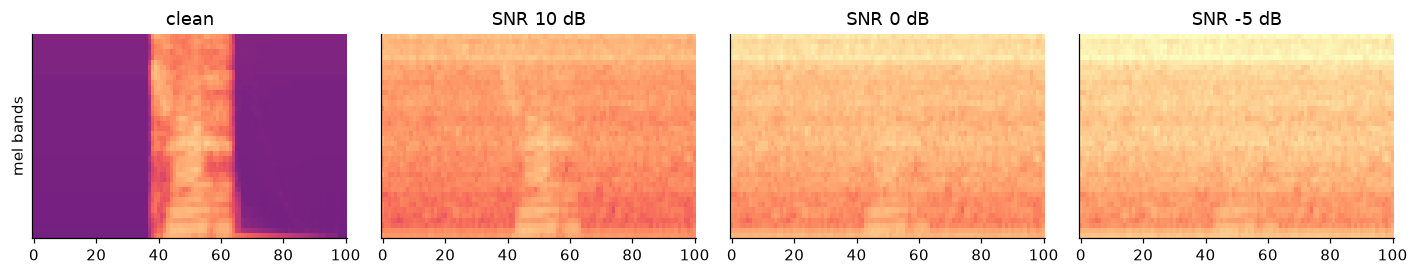
\includegraphics[width=\columnwidth]{logmel_ruido.png}
\caption{Espectrograma log-mel de un clip de ``tres'' limpio y con ruido a distintas SNR.}
\label{fig:logmel}
\end{figure}

\section{Modelo}
\subsection{Arquitectura}
La Figura~\ref{fig:arq} muestra la arquitectura. El codificador tiene tres bloques con 32, 64 y 128 canales. Cada bloque aplica dos veces la secuencia convolución $3 \times 3$, normalización por lotes \cite{b9} y ReLU, y termina con un max pooling de $2 \times 2$.

El clasificador aplica promedio global (global average pooling) a la representación latente, dropout de 0.3 y una capa densa de 22 salidas con softmax. El decodificador aplica tres convoluciones transpuestas con 64, 32 y 16 canales y paso 2, cada una con normalización por lotes y ReLU, un reescalado a $40 \times 101$ y una convolución final de un canal que produce el espectrograma reconstruido. El decodificador solo se usa durante el entrenamiento.

\begin{figure*}[htbp]
\centering
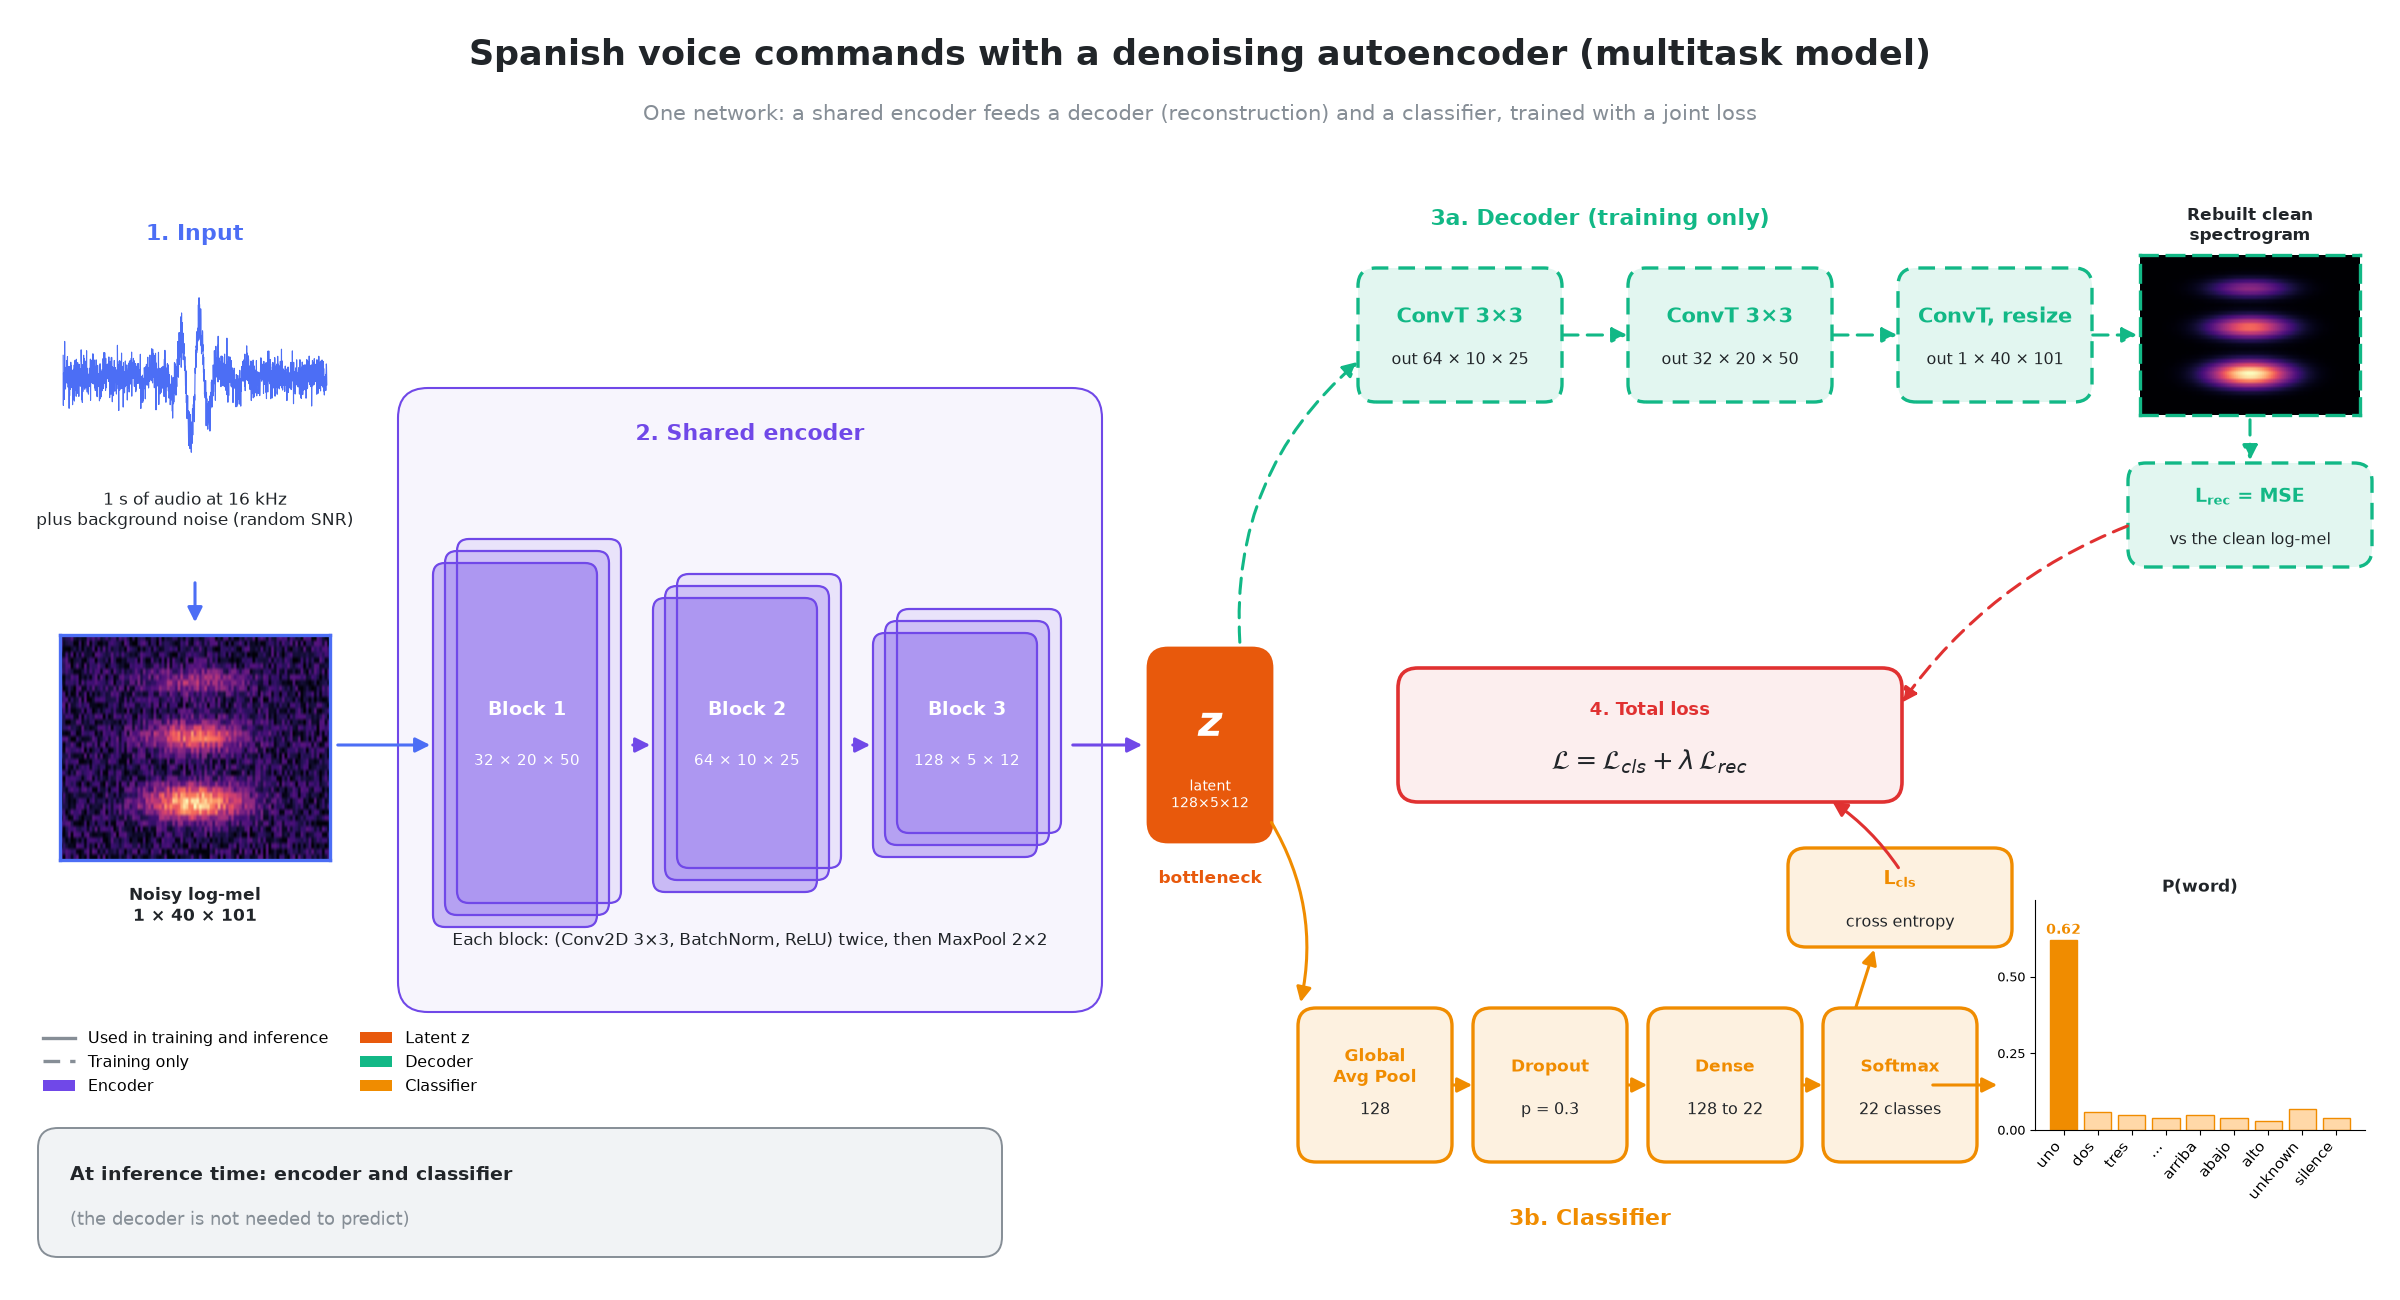
\includegraphics[width=\textwidth]{architecture.png}
\caption{Arquitectura del modelo. El codificador compartido alimenta al clasificador y, durante el entrenamiento, al decodificador.}
\label{fig:arq}
\end{figure*}

\subsection{Función de pérdida}
Las dos salidas se entrenan de forma conjunta con la pérdida de la ecuación~\ref{eq:perdida}. $\mathcal{L}_{cls}$ es la entropía cruzada de la clasificación y $\mathcal{L}_{rec}$ es el error cuadrático medio entre el espectrograma reconstruido y el log-mel normalizado del audio limpio. La entrada de la red siempre es el audio con ruido, por lo que el decodificador aprende a eliminarlo. El hiperparámetro $\lambda = 0.3$ controla el peso de la reconstrucción.
\begin{equation}
\mathcal{L} = \mathcal{L}_{cls} + \lambda \, \mathcal{L}_{rec}
\label{eq:perdida}
\end{equation}

\subsection{Entrenamiento}
El ruido se agrega al vuelo cada vez que se arma un lote, de modo que el modelo casi nunca ve el mismo clip con el mismo ruido. A cada clip se le aplica un desplazamiento aleatorio en el tiempo de hasta 0.1 s. Con probabilidad de 80\% se mezcla con ruido a una SNR uniforme entre $-5$ y 20 dB, y los clips de silencio siempre llevan ruido; el resto queda limpio. Por último se cambia el volumen entre $-6$ y $+6$ dB, y el objetivo de reconstrucción es el mismo clip limpio con el mismo cambio de volumen. Los clips se muestrean con probabilidad proporcional a $n_c^{-1/2}$, donde $n_c$ es el tamaño de su clase, lo que da más peso a las clases con pocos ejemplos.

El modelo se entrena 30 épocas con lotes de 256 clips usando Adam \cite{b5} con tasa de aprendizaje inicial de $10^{-3}$, que se reduce a la mitad cuando la exactitud de validación deja de mejorar durante 3 épocas. La validación usa el set de dev con ruido del fold 4, y se guardan los pesos de la época con mejor exactitud.

\section{Estado actual}
El código está organizado en un paquete \texttt{src/} con la configuración, la preparación y mezcla de datos, la capa \texttt{LogMel}, el modelo, el entrenamiento y la evaluación. El script \texttt{scripts/train.py} entrena el modelo a partir de ese paquete, y \texttt{main.py} ejecuta el dictado en vivo desde el micrófono con los pesos entrenados, reportando una palabra solo cuando su probabilidad supera 0.6. El código está disponible en el repositorio del proyecto \cite{b8}.

El set de prueba se evalúa con audio limpio y con ruido del fold 5 a SNR de 20, 10, 5, 0 y $-5$ dB. La Tabla~\ref{tab:resultados} resume los resultados. El modelo alcanza 92.7\% de exactitud con audio limpio y 84.7\% de exactitud y 82.2\% de F1 macro en promedio sobre las cinco condiciones con ruido. El desempeño se mantiene hasta 5 dB y disminuye de forma marcada a $-5$ dB.

\begin{table}[htbp]
\caption{Resultados en el set de prueba (\%)}
\label{tab:resultados}
\centering
\small
\setlength{\tabcolsep}{3pt}
\begin{tabular}{lcccccc}
\toprule
Métrica & Limpio & 20 dB & 10 dB & 5 dB & 0 dB & $-5$ dB \\
\midrule
Exactitud & 92.7 & 91.8 & 89.7 & 87.5 & 82.4 & 72.3 \\
F1 macro & 92.0 & 91.2 & 88.0 & 85.2 & 79.6 & 67.2 \\
\bottomrule
\end{tabular}
\end{table}

Como siguientes pasos se plantea comparar contra una red de la misma arquitectura sin decodificador, para determinar si la reconstrucción mejora la clasificación, analizar los errores por clase y evaluar otros valores de $\lambda$.

\begin{thebibliography}{00}
\bibitem{b1} I. Goodfellow, Y. Bengio y A. Courville, \textit{Deep Learning}. MIT Press, 2016.
\bibitem{b2} M. Mazumder \textit{et al.}, ``Multilingual Spoken Words Corpus,'' en \textit{NeurIPS Datasets and Benchmarks Track}, 2021.
\bibitem{b3} K. J. Piczak, ``ESC: Dataset for Environmental Sound Classification,'' en \textit{Proc. 23rd ACM International Conference on Multimedia}, pp. 1015--1018, 2015.
\bibitem{b4} P. Vincent, H. Larochelle, Y. Bengio y P.-A. Manzagol, ``Extracting and composing robust features with denoising autoencoders,'' en \textit{Proc. 25th International Conference on Machine Learning}, pp. 1096--1103, 2008.
\bibitem{b5} D. P. Kingma y J. Ba, ``Adam: A method for stochastic optimization,'' arXiv:1412.6980, 2014.
\bibitem{b6} R. Caruana, ``Multitask learning,'' \textit{Machine Learning}, vol. 28, pp. 41--75, 1997.
\bibitem{b7} P. Warden, ``Speech Commands: A dataset for limited-vocabulary speech recognition,'' arXiv:1804.03209, 2018.
\bibitem{b9} S. Ioffe y C. Szegedy, ``Batch normalization: Accelerating deep network training by reducing internal covariate shift,'' arXiv:1502.03167, 2015.
\bibitem{b8} Repositorio del proyecto: \url{https://github.com/Facundo-Barbera/comandos-de-voz-es}
\end{thebibliography}
\end{document}
